\documentclass{report}


%%%%%%%%%%%%%%%%%%
%   Liste des packages utilisés  %
%%%%%%%%%%%%%%%%%%

% (oui y'en a 95% qui sont inutiles ^^)

\usepackage{amssymb}
\usepackage{array}
\usepackage{hyperref}
\usepackage{booktabs}
\usepackage{multirow}
\usepackage{float}
\usepackage{lmodern} %Pack de police
\usepackage{color}
\usepackage[dvipsnames]{xcolor}
\usepackage{graphicx}
\usepackage[utf8x]{inputenc}
\usepackage[T1]{fontenc}
\usepackage{natbib}
\usepackage[francais]{babel}
\usepackage{caption}
\usepackage{listings}
\usepackage{booktabs}
\usepackage[top=2cm, bottom=2cm,left=2cm, right=2cm]{geometry}
\usepackage{blindtext}
\usepackage{setspace}
\usepackage{graphicx}
\usepackage{titlesec, blindtext, color} % titres spéciaux + couleur pour les chapter

% on transforme les chapters en juste le numéro suivi du titre, avec un barre grisse
\definecolor{gray75}{gray}{0.75}
\newcommand{\hsp}{\hspace{20pt}}
\titleformat{\chapter}[hang]{\Huge\bfseries}{\thechapter\hsp\textcolor{gray75}{|}\hsp}{0pt}{\Huge\bfseries}

\begin{document}


%%%%%%%%%%%
%  Page de garde  %
%%%%%%%%%%%
\begin{titlepage}
	\begin{center}
	
		\begin{spacing}{1.5}
			Projet Picross\\
			\vspace*{\fill}
		\end{spacing}
		
		\begin{spacing}{2.5}
			\textbf{\Huge Application de création et d'aide à la résolution de puzzle \textit{picross}}\\[0.5cm]
			\textbf{\huge Cahier d'analyse et conception} \\
			\vspace*{\fill}
			\textit{Étudiants :}
		\end{spacing}

		\begin{spacing}{1.15}
			\large
			\textsc{Brinon} Baptiste\\
			\textsc{Brocherieux} Thibault\\
			\textsc{Cohen} Mehdi\\
			\textsc{Debonne} Valentin\\
			\textsc{Lardy} Anthony\\
			\textsc{Mottier} Emeric\\
			\textsc{Pastouret} Gilles\\
			\textsc{Pelloin} Valentin\\
			\vspace*{\fill}
			\textbf{Groupe n°2} \\
			\textnormal{\large Licence Informatique\\ Le Mans Université\\ \today}
		\end{spacing}
		
	\end{center}
\end{titlepage}


%%%%%%%%%%
%    Sommaire    %
%%%%%%%%%%
\renewcommand{\contentsname}{Sommaire}
\tableofcontents


\chapter{Présentation}

	\section{Introduction}

		Dans le cadre de l'unité d'enseignement "Génie logiciel 2" de la Licence d'informatique de Le Mans Université, les étudiants de troisième année sont amenés à travailler sur un projet de développement d'une application. \\
		Ce document permet de présenter les solutions au cahier des charges, ainsi que l'architecture du programme demandé. Celui-ci est composé en plusieurs parties : la gestion d'une partie, l'aide à la résolution du picross, la gestion des statistiques du joueur (scores, niveaux débloqués, ...) ainsi qu'une interface graphique permettant l'utilisation de ces fonctionnalités. Ce document décrit aussi l'utilisation du temps qui nous est imparti. 

	
 	\section{Objectif de l'application}		
		Nous devons réaliser un jeu de type picross (aussi appelé \textit{nonogramme}, logigramme ou \textit{hanjie}) permettant à un utilisateur de résoudre des grilles et de l'aider dans sa réalisation.
		
	\section{Outils}
		
		Afin de réaliser notre application de \textit{picross}, nous utilisons plusieurs outils. Ruby est le langage utilisé pour programmer le logiciel, incluant une documentation généré par \textit{RDoc} et l'utilisation des bibliothèques de \textit{GTK} pour la réalisation des interfaces graphiques.
LaTeX est utilisé pour rédiger et mettre en forme les différents livrables avant de les convertir en format PDF.
Git et GitHub permettent le partage d'informations et la mise en commun du code ainsi que les livrables associés. Nous nous servons de Discord afin de communiquer au sein du groupe afin de partager nos idées, nos informations et notre travail.
Pour concevoir les différents diagrammes UML, nous avons recours au logiciel Astah et au site internet Tom's Planner.
Afin de créer les maquettes du logiciel (disponibles en Annexe) permettant d’avoir un rendu de la future interface graphique, nous avons utilisé le logiciel Balsamiq.
Pour simplifier la vérification de la qualité du code produit, nous utilisons Code Climate (maintenabilité) ainsi que Travis CI(compilation et tests).

		
\chapter{Conception générale}

    \section{Diagramme de Gantt détaillé}
    
    \begin{figure}[H]
	\caption{Diagramme de \textit{Gant détaillé}}
	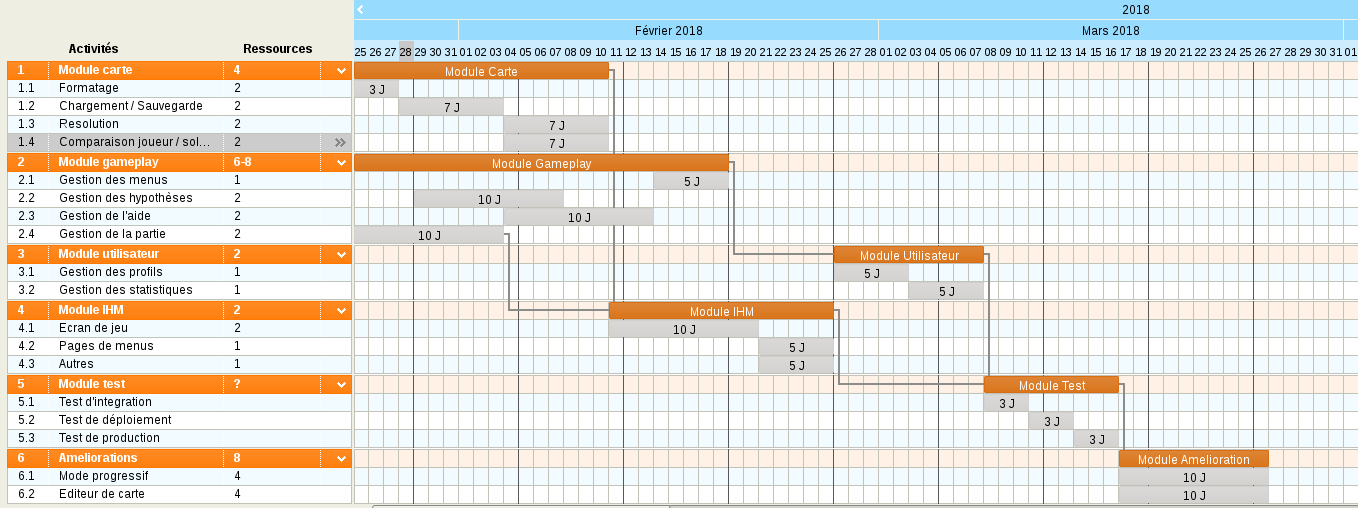
\includegraphics[width=17cm]{ganttDetaille.png}
    \end{figure}
   
     À travers ce diagramme de Gantt, nous observons l'organisation du projet sur les trois mois à venir. Le projet se découpe en plusieurs modules : carte, gameplay, utilisateur, IHM, test et améliorations.
    Chaque module a une durée de vie, nous lui accordons un temps de travail et un certain nombre de personnes, les modules sont également divisés en différentes étapes ce qui correspond aux fonctionnalités de l'application. Les modules sont imbriqués les uns dans les autres, c'est-à-dire que certains dépendent d'autres modules. Sans les modules gameplay et carte réalisés, le module IHM ne peut être réalisé. 
    
    \section{Diagramme de cas d'utilisations}
      
    \begin{figure}[H]
	\caption{Diagramme de \textit{Cas d’utilisation}}
	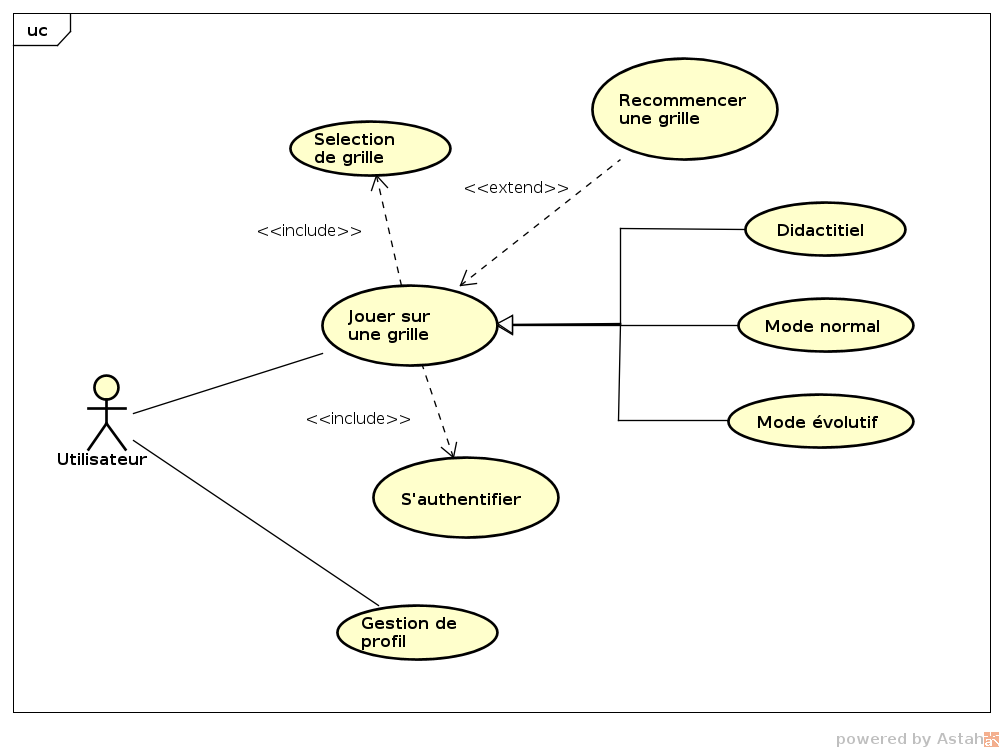
\includegraphics[width=17cm]{../UML/UseCase_diagram/UseCase1.png}
    \end{figure}
    
      %Description des cas d'utilisation

	Le but de l'utilisateur est de jouer sur une grille de \textit{picross}.
Pour cela, il doit avoir un profil. Il peut donc en créer un nouveau s'il en a envie, ou s'authentifier à un profil déjà existant.
	Le joueur doit ensuite sélectionner une grille à l'aide du menu. Il a le choix entre trois types de jeu :
	\begin{itemize}
	\item Le didacticiel, permettant d'apprendre les règles du jeu. 
	\item Le mode classique, permettant de jouer sur plusieurs grilles de tailles et difficultés variables.
	\item Le mode évolutif, agrandissant la taille de la grille au fur et à mesure que le joueur résoudra celle-ci.
	\end{itemize}
	À tout moment, celui-ci peut utiliser l'aide intégrée au jeu pour se débloquer. Il peut aussi choisir de recommencer la grille s'il le souhaite.

      
	\section{Partie classique}
		Dans le mode classique, le joueur a accès à plusieurs fonctionnalités. Il doit tout d'abord choisir un chapitre débloqué puis une grille. Ensuite, quand il se trouve en partie, il peut tout d'abord interagir avec la grille en cochant une case afin de se repérer dans les cases qui ne doivent pas être coloriées ou en coloriant une case. Il peut également enlever une coche ou une couleur d'une case s'il s'aperçoit qu'il s'est trompé. Il peut aussi sélectionner un groupe de cases à colorier, cocher ou vider. \\
		Au niveau de l'interface, l'utilisateur peut, à l'aide de boutons, réinitialiser la grille s'il souhaite repartir de zéro ou la valider s'il pense l'avoir finie. S'il la réussit, il sera renvoyé dans le chapitre en cours. Il peut également utiliser différentes aides (en cliquant sur un bouton) qui diffèrent par la clarté de l'indice, leur coût et leur pénalité. Enfin, l'utilisateur peut quitter la partie quand il le souhaite, la grille est sauvegardée automatiquement.
	
	\section{Parties evolutives}
	
	Lors d'une partie en mode évolutif, le joueur choisit une des grilles du mode avec une taille fixe de 5x5 (cases). Pour résoudre cette grille, il a accès aux mêmes fonctionnalités qu'une partie classique soit interagir avec la grille et avec l'interface. \\
Une fois la grille réussie, celle-ci évolue en une grille plus grande (10x10) tout en gardant le coin supérieur gauche identique à la grille 5x5 réalisée par l'utilisateur (voir exemple en Annexe). Après cela, le joueur doit remplir la grille 10x10 en ayant les mêmes fonctionnalités que précédemment puis la grille évolue une nouvelle fois en 15x15 et ainsi de suite jusqu'à atteindre la taille maximale de 25x25. Une fois la grille 25x25 réussie, le joueur gagne la partie et est renvoyé sur le choix de la grille.
	
	% schéma exemple partie évolutive
	
	\section{Didacticiel}
	
	Une partie en mode didacticiel est une partie guidée afin que l'utilisateur comprenne la logique de résolution d'une partie de \textit{picross}. Les mouvements de celui-ci sont donc restreint aux coups (cocher ou colorier) que lui dit de jouer l'application.
	
  \section{Aides}

  L'utilisateur possède un nombre d'aides gratuites quand il commence à jouer et peut en récupérer en terminant un certain nombre de grille. Quand il est en jeu, il peut les utiliser afin de se débloquer sans pénalité de temps. S'il ne possède plus d'aides gratuites, alors il peut continuer d'utiliser l'aide, mais celle-ci aura un coût (en temps) proportionnel à la difficulté du picross qui sera appliqué à chaque utilisation. La difficulté influence aussi le type d'aide appliqué:
    \begin{itemize}
    \item En mode facile : coloriage de toute une ligne ou colonne
    \item En mode normal : coloriage d'une case correcte 
    \item En mode difficile : indication d'une ligne ou colonne où se trouve une case correcte non coloriée
    \end{itemize}


  \section{IHM}
  
  Les maquettes de l'interface sont accessibles en Annexe.
  
  
			
\chapter{Conception détaillé}

    \section{Diagramme de classe}
    
    \begin{figure}[H]
	\caption{Diagramme de \textit{Classes}}
	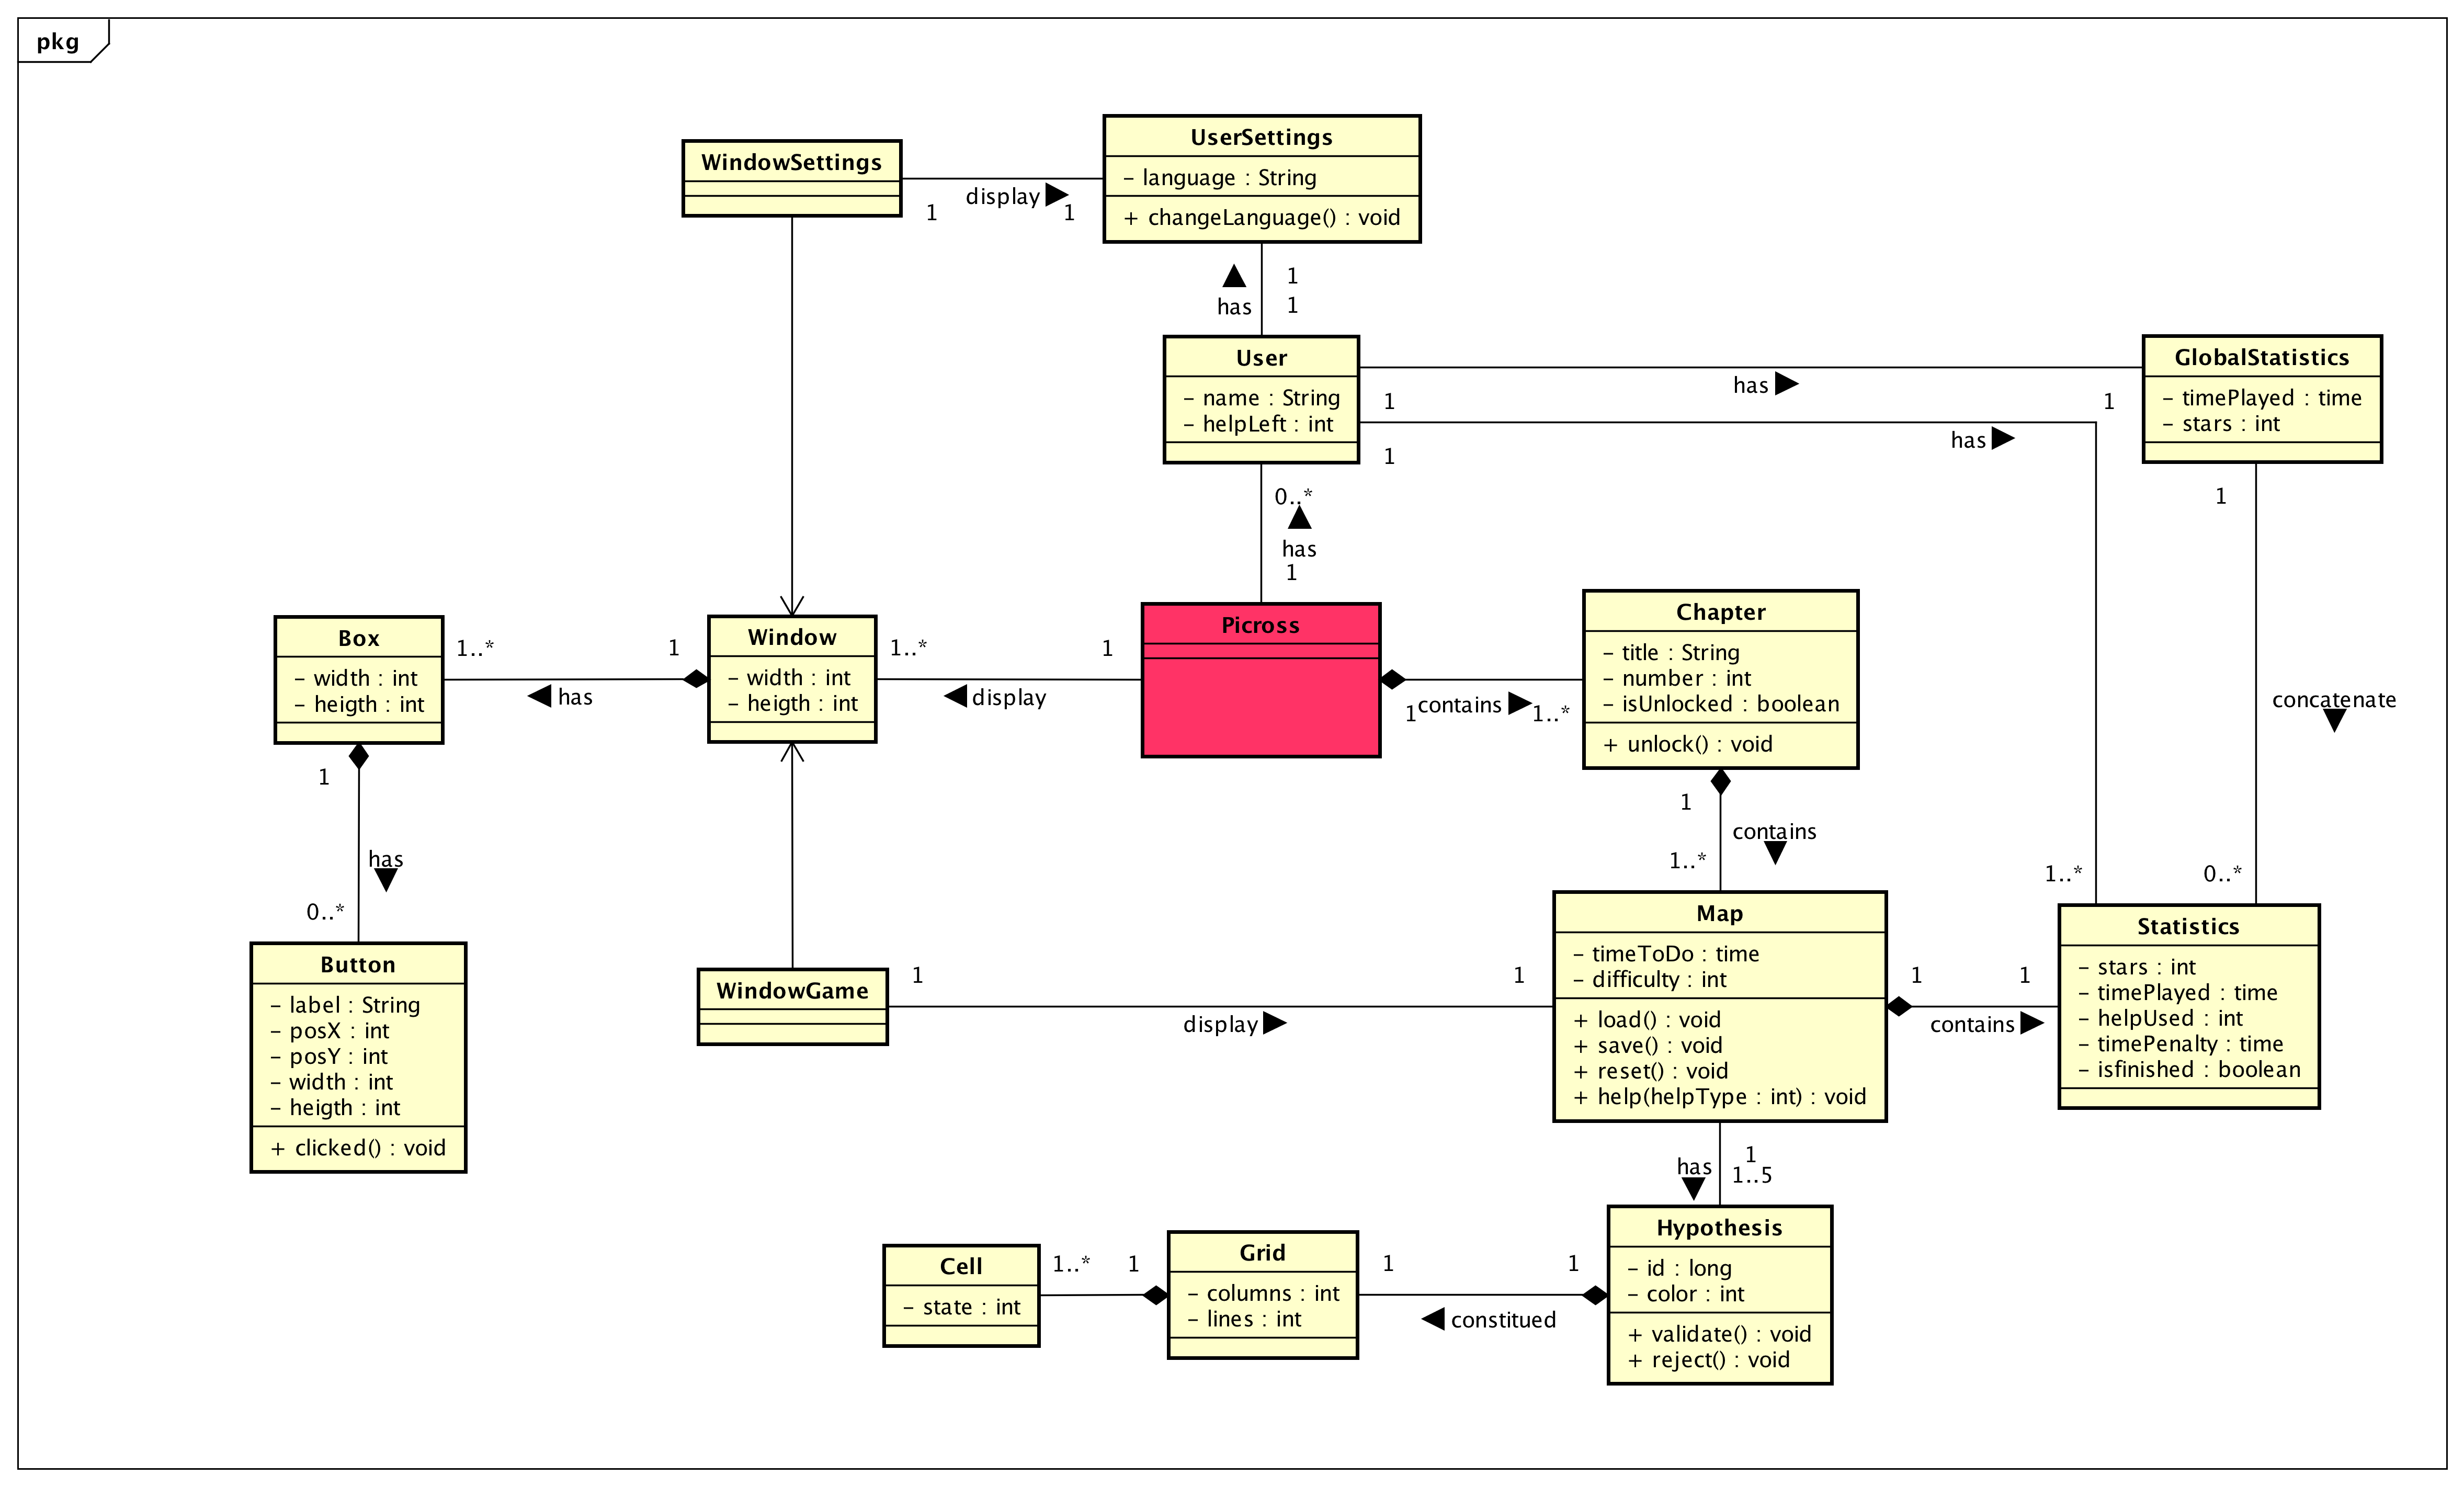
\includegraphics[width=17cm]{../UML/Class_Diagram/DiagrammeClasse.png}
    \end{figure}
    
    	
	Le diagramme de classe ci-dessus présente les différentes classes que nous allons implémenter afin de programmer notre application. Nous avons tout d’abord la classe \textit{picross} qui est la racine permettant de rassembler toutes les autres classes et qui représente l’ensemble du jeu. Cette classe est liée à 3 modules principaux : l’Interface Homme-Machine, les données utilisateur, ainsi que le système de jeu.

	L’IHM commence par la classe Window correspondant à la fenêtre de l’application et possédant une taille définie et modifiable. Cette fenêtre contient plusieurs objets de classe Box possédant chacune une taille définie et représentant les différentes parties graphiques de la fenêtre (la grille, le chronomètre, l’affichage des informations, etc). Chacune de ces boîtes peut contenir des objets de classe Button correspondant aux boutons nécessaires à l’interaction entre l’utilisateur et le logiciel (valider la grille, retourner au menu, etc).

	Les données de l’utilisateur sont rassemblées dans la classe User possédant un pseudo, le nombre d’aides auxquelles il a le droit, et des données séparées en deux parties. La première correspondant aux différents paramètres du logiciel comme la langue utilisée ou la taille de la fenêtre (classe \textit{WindowSetting}) et modélisée grâce à la classe \textit{UserSettings}. La deuxième est liée aux statistiques  générales de l’utilisateur (classe \textit{GlobalStatistics}) comme le temps joué ou le nombre total d’étoiles ainsi que les statistiques liées à chaque grille finie par le joueur (classe \textit{Statistics}) comme le nombre d’étoiles reçues, le temps mis à la finir ainsi que le nombre d’aides utilisées.

 	Le système de jeu est rassemblé dans la classe \textit{Chapter} possédant un titre et un numéro ainsi qu’un booléen indiquant si ce chapitre est verrouillé ou non. Chaque chapitre est composé de plusieurs grilles représentées dans le diagramme par la classe \textit{Map} possédant une difficulté ainsi que le temps de base à réaliser la grille permettant ensuite de calculer le nombre d’étoiles obtenues par le joueur en fonction de son temps. Chacun de ses objets Map est capable de réaliser plusieurs actions comme s’initialiser, sauvegarder ou se réinitialiser. Lors d’une partie sur une grille, l’utilisateur peut utiliser le mode hypothèse représenté par la classe \textit{Hypothesis} composé d’un numéro et d’une couleur. Chacune de ses hypothèses est composée d’une sauvegarde de la grille (classe \textit{Grid}) avec l’état de chaque case (colorié, non colorié, croix) représenté par la classe \textit{Cell}.


\chapter{Annexes}

	\section{Exemple partie évolutive}
	
	\begin{figure}[H]
    		\begin{minipage}[c]{.46\linewidth}
        		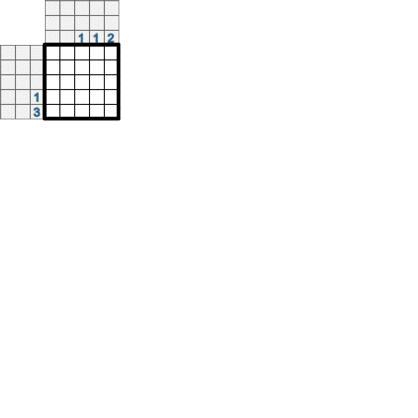
\includegraphics[width=5cm]{../Images/cat/cat1.png}
       			 \caption{Grille 5x5}
    		\end{minipage}

    		\begin{minipage}[c]{.46\linewidth}
        		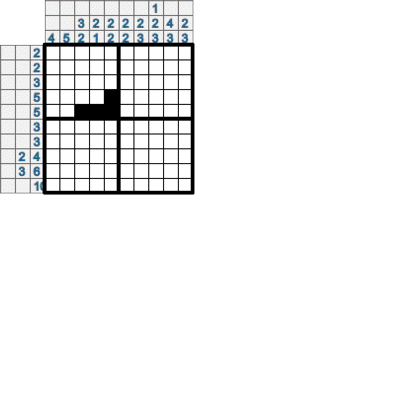
\includegraphics[width=5cm]{../Images/cat/cat2.png}
			\caption{Grille 10x10}
	    	\end{minipage}

		\begin{minipage}[c]{.46\linewidth}
			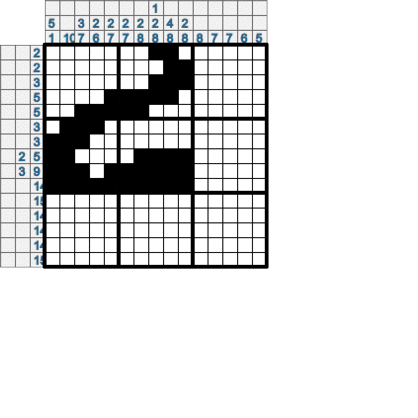
\includegraphics[width=5cm]{../Images/cat/cat3.png}
			\caption{Grille 15x15}
		\end{minipage}
	\end{figure}

	\\
	\begin{figure}[H]
		\begin{minipage}[c]{.46\linewidth}
			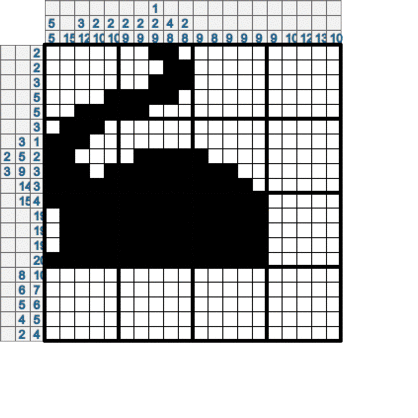
\includegraphics[width=5cm]{../Images/cat/cat4.png}
			\caption{Grille 20x20}
		\end{minipage}

		\begin{minipage}[c]{.46\linewidth}
			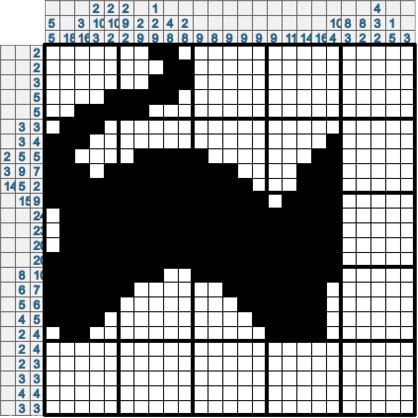
\includegraphics[width=5cm]{../Images/cat/cat5.png}
			\caption{Grille 25x25}
		\end{minipage}
	\end{figure}

	
	\section{Maquettes de l'interface}
      
      		% maquettes

\end{document}
